\documentclass{article}
\usepackage{amsmath,amssymb}
\usepackage{xcolor}
\usepackage{tikz}
\pagestyle{empty}
\pdfpagewidth=1100pt\pdfpageheight=700pt
\begin{document}
\usetikzlibrary{arrows.meta,calc,patterns,positioning,decorations.pathreplacing}

\newcommand{\geometrybandat}[5]{
  \path[band#4] (#2,{#1-.20}) rectangle (#3,{#1+.20});
  \node[font=\scriptsize] at ({#5},#1) {$#4$};
}
\newcommand{\geometryband}[4]{
  \geometrybandat{#1}{#2}{#3}{#4}{(#2+#3)/2}
}
\newcommand{\geometryrow}[2]{
  \node[anchor=east,align=right,font=\scriptsize]
    at (-8.20,#1) {#2};
}
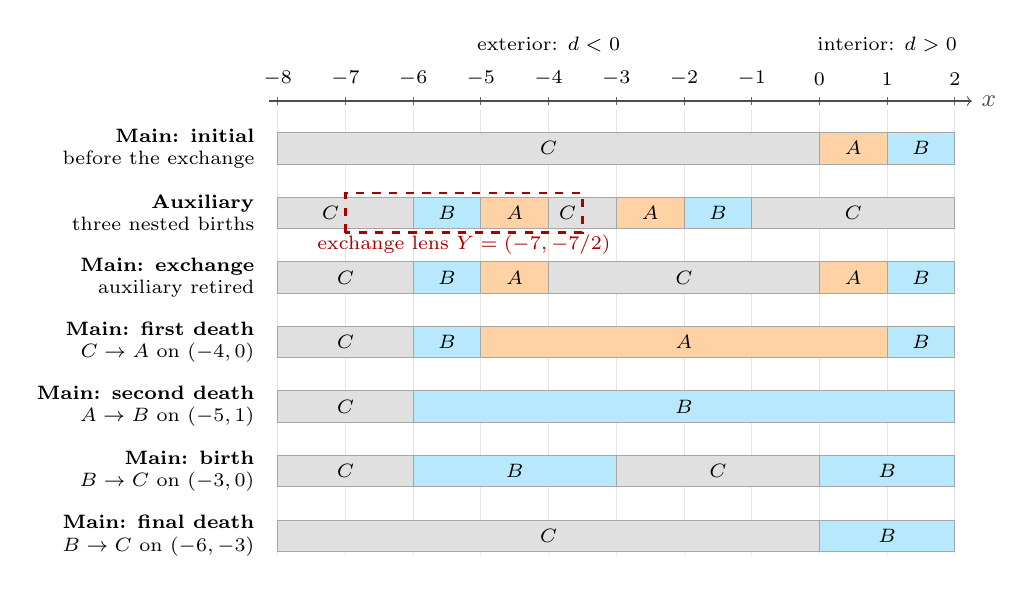
\begin{tikzpicture}[
  x=.86cm,y=1cm,
  bandA/.style={fill=orange!35,draw=black!35,line width=.3pt},
  bandB/.style={fill=cyan!28,draw=black!35,line width=.3pt},
  bandC/.style={fill=black!12,draw=black!35,line width=.3pt},
  lens/.style={draw=red!65!black,dashed,line width=.8pt}
]
  \foreach \geometrytick in {-8,-7,...,2} {
    \draw[black!10,line width=.3pt]
      (\geometrytick,.48) -- (\geometrytick,-5.17);
    \draw[black!60,line width=.35pt]
      (\geometrytick,.55) -- (\geometrytick,.65);
    \node[above,font=\scriptsize] at (\geometrytick,.67)
      {$\geometrytick$};
  }
  \draw[->,black!70] (-8.13,.60) -- (2.25,.60)
    node[right,font=\small] {$x$};
  \node[font=\scriptsize] at (-4,1.32) {exterior: $d<0$};
  \node[font=\scriptsize] at (1,1.32) {interior: $d>0$};

  
  \node[anchor=east,align=right,font=\scriptsize]
    at (-8.20,0) {\textbf{Main: initial}\\before the exchange};

  
  
  \path[bandC] (-8,{0-.20}) rectangle (0,{0+.20});
  \node[font=\scriptsize] at ({(-8+0)/2},0) {$C$};


  
  
  \path[bandA] (0,{0-.20}) rectangle (1,{0+.20});
  \node[font=\scriptsize] at ({(0+1)/2},0) {$A$};


  
  
  \path[bandB] (1,{0-.20}) rectangle (2,{0+.20});
  \node[font=\scriptsize] at ({(1+2)/2},0) {$B$};



  
  \node[anchor=east,align=right,font=\scriptsize]
    at (-8.20,-.82) {\textbf{Auxiliary}\\three nested births};

  
  \path[bandC] (-8,{-.82-.20}) rectangle (-6,{-.82+.20});
  \node[font=\scriptsize] at ({-7.22},-.82) {$C$};

  
  
  \path[bandB] (-6,{-.82-.20}) rectangle (-5,{-.82+.20});
  \node[font=\scriptsize] at ({(-6+-5)/2},-.82) {$B$};


  
  
  \path[bandA] (-5,{-.82-.20}) rectangle (-4,{-.82+.20});
  \node[font=\scriptsize] at ({(-5+-4)/2},-.82) {$A$};


  
  \path[bandC] (-4,{-.82-.20}) rectangle (-3,{-.82+.20});
  \node[font=\scriptsize] at ({-3.72},-.82) {$C$};

  
  
  \path[bandA] (-3,{-.82-.20}) rectangle (-2,{-.82+.20});
  \node[font=\scriptsize] at ({(-3+-2)/2},-.82) {$A$};


  
  
  \path[bandB] (-2,{-.82-.20}) rectangle (-1,{-.82+.20});
  \node[font=\scriptsize] at ({(-2+-1)/2},-.82) {$B$};


  
  
  \path[bandC] (-1,{-.82-.20}) rectangle (2,{-.82+.20});
  \node[font=\scriptsize] at ({(-1+2)/2},-.82) {$C$};


  \draw[lens] (-7,-1.07) rectangle (-3.5,-.57);
  \node[below,inner sep=0pt,font=\scriptsize,text=red!65!black] at (-5.25,-1.09)
    {exchange lens $Y=(-7,-7/2)$};

  
  \node[anchor=east,align=right,font=\scriptsize]
    at (-8.20,-1.64) {\textbf{Main: exchange}\\auxiliary retired};

  
  
  \path[bandC] (-8,{-1.64-.20}) rectangle (-6,{-1.64+.20});
  \node[font=\scriptsize] at ({(-8+-6)/2},-1.64) {$C$};


  
  
  \path[bandB] (-6,{-1.64-.20}) rectangle (-5,{-1.64+.20});
  \node[font=\scriptsize] at ({(-6+-5)/2},-1.64) {$B$};


  
  
  \path[bandA] (-5,{-1.64-.20}) rectangle (-4,{-1.64+.20});
  \node[font=\scriptsize] at ({(-5+-4)/2},-1.64) {$A$};


  
  
  \path[bandC] (-4,{-1.64-.20}) rectangle (0,{-1.64+.20});
  \node[font=\scriptsize] at ({(-4+0)/2},-1.64) {$C$};


  
  
  \path[bandA] (0,{-1.64-.20}) rectangle (1,{-1.64+.20});
  \node[font=\scriptsize] at ({(0+1)/2},-1.64) {$A$};


  
  
  \path[bandB] (1,{-1.64-.20}) rectangle (2,{-1.64+.20});
  \node[font=\scriptsize] at ({(1+2)/2},-1.64) {$B$};



  
  \node[anchor=east,align=right,font=\scriptsize]
    at (-8.20,-2.46) {\textbf{Main: first death}\\$C\to A$ on $(-4,0)$};

  
  
  \path[bandC] (-8,{-2.46-.20}) rectangle (-6,{-2.46+.20});
  \node[font=\scriptsize] at ({(-8+-6)/2},-2.46) {$C$};


  
  
  \path[bandB] (-6,{-2.46-.20}) rectangle (-5,{-2.46+.20});
  \node[font=\scriptsize] at ({(-6+-5)/2},-2.46) {$B$};


  
  
  \path[bandA] (-5,{-2.46-.20}) rectangle (1,{-2.46+.20});
  \node[font=\scriptsize] at ({(-5+1)/2},-2.46) {$A$};


  
  
  \path[bandB] (1,{-2.46-.20}) rectangle (2,{-2.46+.20});
  \node[font=\scriptsize] at ({(1+2)/2},-2.46) {$B$};



  
  \node[anchor=east,align=right,font=\scriptsize]
    at (-8.20,-3.28) {\textbf{Main: second death}\\$A\to B$ on $(-5,1)$};

  
  
  \path[bandC] (-8,{-3.28-.20}) rectangle (-6,{-3.28+.20});
  \node[font=\scriptsize] at ({(-8+-6)/2},-3.28) {$C$};


  
  
  \path[bandB] (-6,{-3.28-.20}) rectangle (2,{-3.28+.20});
  \node[font=\scriptsize] at ({(-6+2)/2},-3.28) {$B$};



  
  \node[anchor=east,align=right,font=\scriptsize]
    at (-8.20,-4.10) {\textbf{Main: birth}\\$B\to C$ on $(-3,0)$};

  
  
  \path[bandC] (-8,{-4.10-.20}) rectangle (-6,{-4.10+.20});
  \node[font=\scriptsize] at ({(-8+-6)/2},-4.10) {$C$};


  
  
  \path[bandB] (-6,{-4.10-.20}) rectangle (-3,{-4.10+.20});
  \node[font=\scriptsize] at ({(-6+-3)/2},-4.10) {$B$};


  
  
  \path[bandC] (-3,{-4.10-.20}) rectangle (0,{-4.10+.20});
  \node[font=\scriptsize] at ({(-3+0)/2},-4.10) {$C$};


  
  
  \path[bandB] (0,{-4.10-.20}) rectangle (2,{-4.10+.20});
  \node[font=\scriptsize] at ({(0+2)/2},-4.10) {$B$};



  
  \node[anchor=east,align=right,font=\scriptsize]
    at (-8.20,-4.92) {\textbf{Main: final death}\\$B\to C$ on $(-6,-3)$};

  
  
  \path[bandC] (-8,{-4.92-.20}) rectangle (0,{-4.92+.20});
  \node[font=\scriptsize] at ({(-8+0)/2},-4.92) {$C$};


  
  
  \path[bandB] (0,{-4.92-.20}) rectangle (2,{-4.92+.20});
  \node[font=\scriptsize] at ({(0+2)/2},-4.92) {$B$};


\end{tikzpicture}
\end{document}
